% !TEX root = ../Thesis.tex
%%
%%  Hochschule für Technik und Wirtschaft Berlin --  Abschlussarbeit
%%
%% Kapitel 2 - Theoretische Grundlagen und Forschungsstand
%%
%%


\chapter{Theoretische Grundlagen} \label{Grundlagen}

In diesem Kapitel werden die nötigen Grundlagen zum Verständnis des Port-\eng{Scannings} in Form von \texttt{SYN}-Scans, sowie 
das nötige Wissen über Netzwerkkommunikation, die genutzten Technologien und Linux-Schnittstellen vermittelt.
Des Weiteren wird auf asynchrone Programmierung eingegangen, sodass ein Verständnis für das nachfolgende Konzept 
der Implementierung gegeben ist.

Anschließend werden die zum Vergleich genutzten Scanner vorgestellt und eingeordnet. Auch Rust und dessen 
Besonderheiten werden genauer vorgestellt.

\section{Grundlagen der Netzwerkkommunikation}
Bei der Kommunikation in TCP/IP \footnote{Eine grundlegende Kenntnis über das TCP/IP-Modell wird angenommen} 
Netzwerken dient das IP-Protokoll und die IP-Adressen der Identifikation der Maschine im Netzwerk, während die genaue 
Adressierung der spezifischen Anwendungen durch sogenannte Ports bzw. der sogenannten Portnummer bestimmt wird \cite{Chapter_4._Port_Scanning_Overview_|_Nmap_Network_Scanning}. 
Die Portnummer ist ein 16-Bit-Wert und kann somit zwischen jeweils einschließlich 0 und 65535 liegen \cite[S.~107]{Computernetzwerke}. Einige Portnummern
sind fest vergeben oder für bestimmte Anwendungen registriert \cite{IANA_Port_Registry}, was es ermöglicht, gezielt nach bestimmten Anwendungen zu scannen.
Der gesamte Kommunikations-Endpunkt wird \eng{Socket} genannt \cite[S.~1149]{Kerrisk_2018}. 

\subsection{Ports}
Ports können in verschiedene Zustände eingeordnet werden. Für diese Arbeit ist nur die Unterscheidung zwischen offen und geschlossen/gefiltert relevant.

\begin{itemize} 
	\item \textbf{Offen:} Eine Anwendung lauscht auf dem Port und akzeptiert eingehende valide 
	TCP oder UDP Anfragen \cite{Lyon_2010}.
	\item \textbf{Geschlossen / Gefiltert:} Der mit dem Port verbundene Service ist zwar ansprechbar, aber akzeptiert keine eingehenden Verbindungen / 
	Es gibt lediglich eine ICMP (Fehler) Antwort oder gar keine, da beispielsweise kein Service für diesen Port
	existiert \cite{Lyon_2010}.
\end{itemize}



\subsection{Transmission Control Protocol (TCP)}
Das \eng{Transmission Control Protocol} operiert in der Transportschicht des TCP/IP-Modells und ist eines der meistgenutzten
Transportprotokolle des Internets \cite[S.~71]{Wendzel_2021}. Es gewährleistet eine zuverlässige, verbindungsorientierte
Datenübertragung zwischen den Prozessen der \eng{Hosts}. Die ursprüngliche Spezifikation erfolgte im RFC 793 \cite{Postel_1981},
welches durch RFC 9293 \cite{Eddy_2022} konsolidiert wurde. Für die Entwicklung eines \texttt{SYN}-Scanners sind insbesondere
der Aufbau des TCP-Headers und der Mechanismus des Verbindungsaufbaues entscheidend. 

\begin{figure}[htbp]
    \centering
    % Skalierung vergrößert (x für Breite, y für Höhe der Zeilen)
    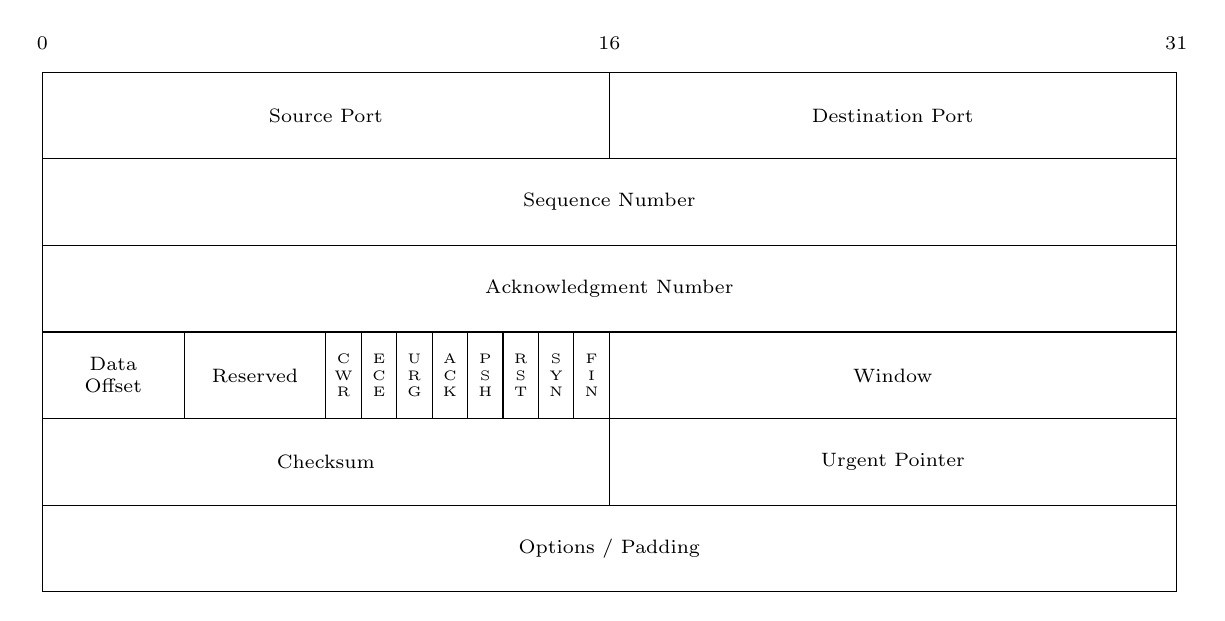
\begin{tikzpicture}[x=0.45cm, y=1.1cm, every node/.style={font=\scriptsize, align=center}]
        % Bit indices - 10 entfernt
        \node[anchor=south] at (0,6.15) {0};
        \node[anchor=south] at (16,6.15) {16};
        \node[anchor=south] at (32,6.15) {31};

        % Row 1: Source / Destination Port
        \draw (0,6) rectangle (16,5) node[midway] {Source Port};
        \draw (16,6) rectangle (32,5) node[midway] {Destination Port};

        % Row 2: Sequence Number
        \draw (0,5) rectangle (32,4) node[midway] {Sequence Number};

        % Row 3: Acknowledgment Number
        \draw (0,4) rectangle (32,3) node[midway] {Acknowledgment Number};

        % Row 4: Offset, Reserved, Flags, Window
        % Data Offset (4 Bits: 0-3)
        \draw (0,3) rectangle (4,2) node[midway] {Data\\Offset};
        
        % Reserved (4 Bits: 4-7) - "Rsrvd" wie in Vorlage
        \draw (4,3) rectangle (8,2) node[midway] {Reserved};

        % Flags (8 Bits: 8-15) - Einzelne Kästchen mit tiny Schrift gestapelt
        \draw (8,3) rectangle (9,2) node[midway, font=\tiny, inner sep=0pt] {C\\W\\R};
        \draw (9,3) rectangle (10,2) node[midway, font=\tiny, inner sep=0pt] {E\\C\\E};
        \draw (10,3) rectangle (11,2) node[midway, font=\tiny, inner sep=0pt] {U\\R\\G};
        \draw (11,3) rectangle (12,2) node[midway, font=\tiny, inner sep=0pt] {A\\C\\K};
        \draw (12,3) rectangle (13,2) node[midway, font=\tiny, inner sep=0pt] {P\\S\\H};
        \draw (13,3) rectangle (14,2) node[midway, font=\tiny, inner sep=0pt] {R\\S\\T};
        \draw (14,3) rectangle (15,2) node[midway, font=\tiny, inner sep=0pt] {S\\Y\\N};
        \draw (15,3) rectangle (16,2) node[midway, font=\tiny, inner sep=0pt] {F\\I\\N};

        % Window (16 Bits: 16-31)
        \draw (16,3) rectangle (32,2) node[midway] {Window};

        % Row 5: Checksum, Urgent Pointer
        \draw (0,2) rectangle (16,1) node[midway] {Checksum};
        \draw (16,2) rectangle (32,1) node[midway] {Urgent Pointer};

        % Row 6: Options / Padding
        \draw (0,1) rectangle (32,0) node[midway] {Options / Padding};
    \end{tikzpicture}
    \caption{Aufbau des TCP-Headers nach RFC 9293 \cite{Eddy_2022}.}
    \label{fig:tcp_header}
\end{figure}

Da das TCP-Protokoll Daten als \eng{Stream} statt einzeln (\eng{Message}) versendet, 
wird vorher eine Verbindung in einem sogenannten \eng{Three-Way-Handshake} aufgebaut \cite{Wendzel_2021} S71/72. 
Bei diesem werden TCP-Pakete mit jeweils unterschiedlichen Werten in den \eng{Control Bits} (\eng{Flags}) 
des TCP-Headers nach dem in \ref{fig:tcp_handshake} beschriebenen Muster ausgetauscht.

\begin{figure}[htbp]
    \centering
    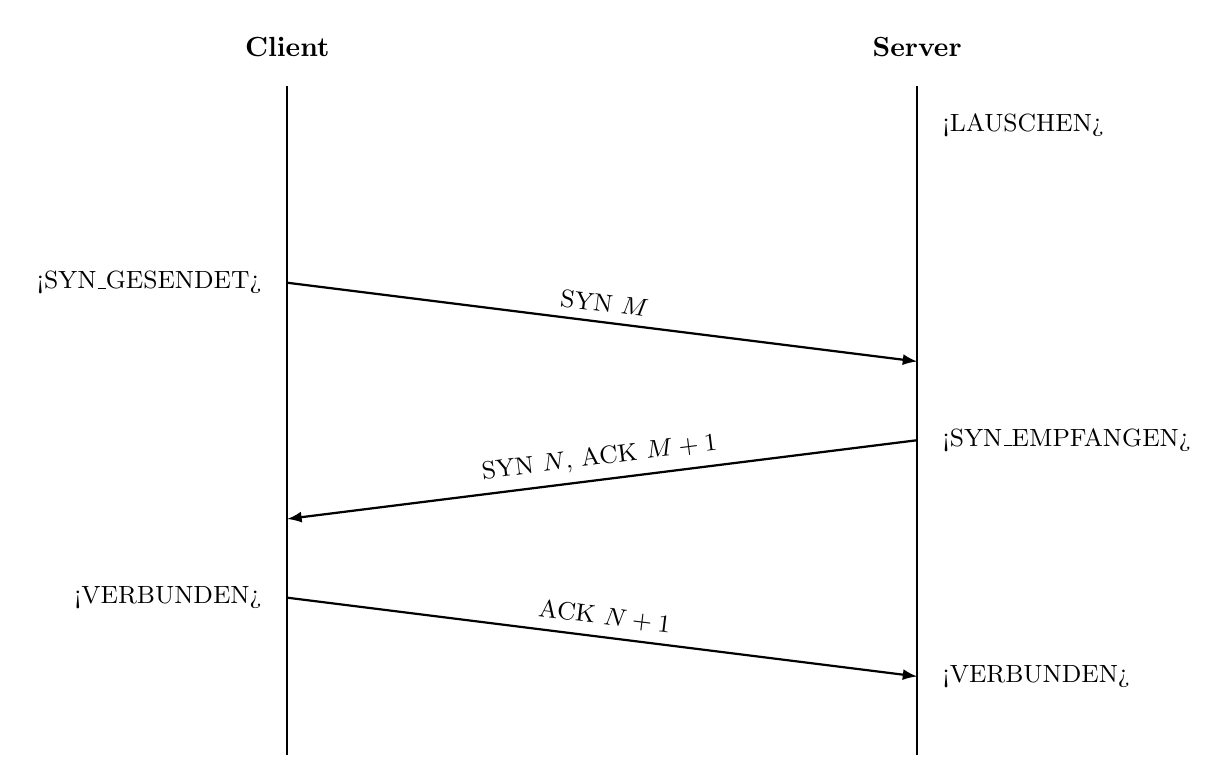
\begin{tikzpicture}[
        >=latex, 
        font=\small,
        node distance=1cm,
        every node/.style={align=center}
    ]

        % --- Koordinaten-Definition ---
        % X-Positionen der Linien
        \def\clientx{0}
        \def\serverx{8}
        
        % Y-Positionen der Ereignisse
        \def\yStart{0}
        \def\yListen{-0.5}
        \def\yConnect{-2}
        \def\ySynSend{-2.5}
        \def\ySynRecv{-3.5}
        \def\ySynAckSend{-4.5}
        \def\ySynAckRecv{-5.5}
        \def\yAckSend{-6.5}
        \def\yAckRecv{-7.5}
        \def\yEnd{-8.5}

        % --- Vertikale Linien (Timelines) ---
        \draw[thick] (\clientx, \yStart) -- (\clientx, \yEnd);
        \draw[thick] (\serverx, \yStart) -- (\serverx, \yEnd);

        % --- Header ---
        \node[font=\bfseries] at (\clientx, 0.5) {Client};
        \node[font=\bfseries] at (\serverx, 0.5) {Server};

        % --- SERVER SEITE (Rechts) ---
        % LISTEN Zustand
        \node[anchor=west] at (\serverx+0.2, \yListen) {<LAUSCHEN>};

        % SYN_RECV Zustand
        \node[anchor=west] at (\serverx+0.2, \ySynAckSend) {<SYN\_EMPFANGEN>};
        
        % ESTABLISHED Zustand
        \node[anchor=west] at (\serverx+0.2, \yAckRecv) {<VERBUNDEN>};


        % --- CLIENT SEITE (Links) ---
        % SYN_SENT Zustand
        \node[anchor=east] at (\clientx-0.2, \ySynSend) {<SYN\_GESENDET>};

        % ESTABLISHED Zustand
        \node[anchor=east] at (\clientx-0.2, \yAckSend) {<VERBUNDEN>};


        % --- NACHRICHTEN (Pfeile) ---
        
        % 1. SYN M
        \draw[->, thick] (\clientx, \ySynSend) -- (\serverx, \ySynRecv) 
            node[midway, above, sloped] {SYN $M$};

        % 2. SYN N, ACK M+1
        \draw[->, thick] (\serverx, \ySynAckSend) -- (\clientx, \ySynAckRecv) 
            node[midway, above, sloped] {SYN $N$, ACK $M+1$};

        % 3. ACK N+1
        \draw[->, thick] (\clientx, \yAckSend) -- (\serverx, \yAckRecv) 
            node[midway, above, sloped] {ACK $N+1$};

    \end{tikzpicture}
    \caption{\eng{Three-Way-Handshake} zum Aufbau einer TCP-Verbindung \cite{Wendzel_2021}.}
    \label{fig:tcp_handshake}
\end{figure}


\section{Portscanning} \label{Portscanning}
Portscanning, als Art des Netzwerkscannings, ist eines der fundamentalen Verfahren in der Netzwerksicherheit zum Auffinden von 
potenziellen Schwachstellen \cite{Chapter_4._Port_Scanning_Overview_|_Nmap_Network_Scanning}. Ein Portscanner verschickt Pakete an ein Zielsystem und
zieht anhand der Antworten, oder auch ausbleibenden Antworten, Rückschlüsse auf den Zustand des Systems. Das Ziel ist die Identifikation
von offenen Ports bzw. aktiven Diensten, was als erster Schritt für weiterführende Sicherheitsanalysen oder aber auch Angriffe dienen kann \cite[S.~4-3]{Scarfone_Souppaya_Cody_Orebaugh_2008}. 

Beim Scannen von Ports können grundsätzlich zwei strategische Ausrichtungen unterschieden werden:
\begin{itemize} 
	\item \textbf{Vertikales Scannen:} Hierbei wird ein einzelner Ziel-\eng{Host}\footnote{Teilnehmer im Netzwerk, der über eine IP-Adresse adressierbar ist.} 
    auf eine Vielzahl von Ports (oft alle 65535) gescannt, um ein möglichst
vollständiges Profil möglicher Schwachstellen des Zielsystems zu erlangen und somit eher für das \eng{Penetration Testing} geeignet ist.
\item \textbf{Horizontales Scannen:} Ein sehr großer Adressbereich, beispielsweise das komplette IPv4-Internet wird gescannt. Dafür ist die Anzahl
der zu scannenden Ports sehr klein oder auf einen einzigen beschränkt. Dies bietet die Möglichkeit wertvolle Daten über Trends oder
die Verbreitung von Schwachstellen zu untersuchen \cite{Durumeric_Wustrow_Halderman}.
\end{itemize} 

% bis hier Rechtschreibung kontrolliert

\subsection{SYN-Scanning}
Für einen \eng{Half-Open} \texttt{SYN}-Scan wie er in dieser Arbeit behandelt wird, sind lediglich die ersten beiden Schritte des in \ref{fig:tcp_handshake} 
dargestellten Verbindungsablaufes relevant. Es wird davon gebraucht gemacht, dass bereits und ausschließlich eine \texttt{SYN/ACK}-Antwort den Port als offen klassifiziert, 
was den weiteren Verbindungsaufbau irrelevant macht \cite{Lyon_2010}. Um den Scan zu verschleiern und den Verbindungsversuch trotz dessen sauber
abzuschießen, kann anschließend noch ein Paket, bei welchem die \texttt{RST}-Flag der \eng{Control Bits} gesetzt ist gesendet werden \cite{Lyon_2010}.

Um antwortende \eng{Hosts} effizient zu identifizieren, wird das Prinzip des \texttt{SYN}-Cookies adaptiert \cite{Durumeric_Wustrow_Halderman}, welches ursprünglich als 
Abwehrmechanismus gegen \eng{Denial-of-Service}-Angriffe spezifiziert wurde \cite[S. 8]{Eddy_2007}. Dafür werden verbindungsspezifische 
Informationen unter Verwendung eines \eng{Hash}-Algorithmus (z. B. \eng{Keyed SipHash} TODO opt. Quelle) kodiert 
und als \eng{Sequence Number} in den TCP-Header des ausgehenden \texttt{SYN}-Pakets eingetragen.
Antwortet ein Ziel-\eng{Host} mit einem \texttt{SYN-ACK}-Paket, so enthält dessen \eng{Acknowledgment Number} gemäß TCP-Spezifikation den inkrementierten 
Wert der ursprünglichen \eng{Sequence Number}. Die Validierung lässt sich abstrahiert wie folgt beschreiben:

\begin{verbatim}is_valid = hash(value_0, value_1, ..., secret) == answer.ack_num - 1\end{verbatim} \label{equ:syn_cookie_auswertung}

Die Validierung der Antwort erfolgt somit rein mathematisch und benötigt keine Speicherung in einer lokalen
Zustandstabelle. Dies erwirkt eine sowohl zeitliche als auch logische Entkopplung von Sende- und Empfangsprozessen,
was wiederum eine asynchrone Architektur ermöglicht.

Entscheidend für den Scanner sind demnach die in \ref{tab:TCP-header-fields} aufgeführten Header Felder. 

\begin{table}[htbp]
\begin{tabularx}{\textwidth}{|c|X|}\hline 
\textbf{Header Feld} & \textbf{Beschreibung} \\ \hline
\eng{Source Port} & Beschreibt den genutzten Port des Ausgangsdienstes. \\ \hline
\eng{Destination Port} &  Beschreibt den zu scannenden Port des Zielsystems. \\ \hline
\eng{Sequence Number} & Wird zur Speicherung des \texttt{SYN}-Cookies genutzt. \\ \hline
\eng{Acknowledgement Number} & Wird zum Abrufen des \texttt{SYN}-Cookies genutzt. \\ \hline
\eng{Control Bits} (\eng{Flags}) & Wird für die verschiedenen Phasen des Verbindungsaufbaues angepasst oder ausgelesen.  \\ \hline
\end{tabularx}
\label{tab:TCP-header-fields}
\caption{Relevante TCP-Header Felder}
\end{table}

\section{Schnittstellen zur Paketverarbeitung unter Linux}
Um einen performanten Scanner zu bauen, müssen die genutzten Technologien zum einen für die Netzwerkprogrammierung 
geeignet und zum anderen hohe Sende- und Empfangsraten zulassen, während möglichst wenig
Rechenressourcen verbraucht werden. 

\subsection{Linux}
Linux ist ein \eng{Open-Source}-Betriebssystem-Kernel \cite[S.~1]{Kerrisk_2018}, welcher aufgrund neuartiger Subsysteme (wie beispielsweise \texttt{eBPF} (siehe \ref{Grundlagen.eBPF}) oder
 \texttt{XDP} (siehe \ref{Grundlagen.XDP})), eine programmierbare Paketverarbeitung nahe an der Hardware ermöglicht. 
 Dies ist für die Entwicklung eines Hochleistungsscanners von großem Vorteil.

Ein zentrales Konzept zum Verständnis der \eng{Performance}-Grenzen ist die Unterscheidung 
zwischen \eng{User Space} und \eng{Kernel Space} im Linux Ökosystem \cite[S.~23]{Kerrisk_2018}: 

\begin{itemize} 
	\item \textbf{\eng{Kernel-Space}:} Hier läuft der Kern des Betriebssystems mit vollem Zugriff 
	auf die Hardware und den Speicher. Treiber und der Netzwerk-Stack operieren auf dieser Ebene. 
	\item \textbf{\eng{User-Space}:} Hier laufen reguläre Anwendungen in isolierten Speicherbereichen. 
	Diese haben keinen direkten Zugriff auf den \eng{Kernel Space}. 
\end{itemize} 
Die Kommunikation zwischen diesen Ebenen erfolgt über \eng{System Calls} \cite[S.~44]{Kerrisk_2018}. Jeder Wechsel (\eng{Context Switch}) 
zwischen \eng{User}- und \eng{Kernel Space}, sowie das Kopieren von Daten zwischen diesen 
Speicherbereichen, erzeugt \eng{Overhead}. Beim Versenden und Empfangen sehr vieler Pakete 
summiert sich dieser \eng{Overhead}, da jedes Paket im Normalfall sowohl \eng{Kernel Space}, als auch \eng{User Space}, 
durchschreitet. Dies belastet die CPU und wird für den Durchsatz zum Flaschenhals \cite{Høiland-Jørgensen_Brouer_Borkmann_Fastabend_Herbert_Ahern_Miller_2018}.

\subsection{\eng{Raw-Sockets} und \eng{Address Families}}
Als Endpunkt für die Kommunikation werden \eng{Sockets} genutzt \cite{socket2_linux_manpage}. Die traditionelle 
Netzwerkprogrammierung unter Linux abstrahiert die Komplexität der Netzwerkprotokolle wie TCP. So übernimmt der Kernel
dabei vollständig den \eng{Three-Way-Handshake} und die Zustandsverwaltung \cite[S.~1158]{Kerrisk_2018}. 
Für einen \texttt{SYN}-Scanner ist dies ungeeignet, da der Scanner lediglich das initiale \texttt{SYN}-Paket senden und die Antwort 
registrieren will, ohne eine vollwertige Verbindung aufzubauen, welche Ressourcen im Kernel binden würde.

\eng{Raw-Sockets} erlauben der Anwendung, Netzwerkpakete unter Umgehung bestimmter \eng{Layer} des Kernel-Stacks zu senden 
und zu empfangen \cite{raw7_linux_manpage}. Der Entwickler muss die Protokoll-Header selbst konstruieren. 
Dies ist für \eng{Half-Open} Portscanner essenziell, um individuelle Pakete zu generieren, ohne dass der Kernel 
automatisch in den Verbindungsaufbau eingreift. 

% TODO eindeutschen
Die \eng{Address Families} definieren dabei die Interpretation der Adressen und die Ebene des Zugriffs \cite{address_families7_linux_manpage}. 
Der Linux-Kernel stellt diverse Address-Familien bereit. Zum Verständnis, im Rahmen dieses Projektes, sind folgende Varianten von zentraler 
Bedeutung:

\begin{itemize} 
	\itemsep 0pt
	\item \textbf{\texttt{AF\_INET} (Netzwerk-Ebene):} Diese Familie operiert auf Layer 3 der IP-Ebene \cite{raw7_linux_manpage}. Bei Nutzung von \eng{Raw-Sockets} fügt der Kernel 
    standardmäßig den IP-Header hinzu und übernimmt das vollständige Routing zur korrekten Netzwerkschnittstelle \cite[S.~1202]{Kerrisk_2018}.
 	\item \textbf{\texttt{AF\_PACKET} (Sicherungsschicht):} Diese Familie ermöglicht direkten Zugriff auf Layer 2 (Ethernet-Ebene). 
	Anwendungen erzeugen vollständige \eng{Ethernet-Frames} und haben somit die volle Kontrolle.
    Das Versenden oder Empfangen von Paketen erfordert jedoch weiterhin die Allokation von Kernel-internen Datenstrukturen \cite{packet_7_-_Linux_manual_page}.
    \item \textbf{\texttt{AF\_XDP} (Hochperformant):} Hierbei handelt es sich um eine speziell für Hochleistungsanwendungen optimierte \eng{Address Family}.
	Sie ermöglicht das Senden und Empfangen von Paketen unter Umgehung des regulären Kernel-Netzwerkstacks. Dabei ist zwischen dem universell verfügbaren \eng{Copy-Mode},
    in welchem Daten zwischen Kernel und User Space kopiert werden und dem Treiber-abhängigen \eng{Zero-Copy-Mode}, in welchem Daten direkt in den Speicher der 
    Anwendung geschrieben werden zu unterscheiden \cite{Høiland-Jørgensen_Brouer_Borkmann_Fastabend_Herbert_Ahern_Miller_2018}. 
\end{itemize}

\subsection{Erweiterte Berkeley Packet Filter (\texttt{eBPF})} \label{Grundlagen.eBPF}
Ursprünglich als \textit{Berkeley Packet Filter} (\texttt{BPF}) für Werkzeuge wie \texttt{tcpdump} entwickelt, um Pakete effizient zu filtern \cite{260309}, 
wurde die Technologie erweitert, sodass grundlegend neue Möglichkeiten außerhalb des reinen filtern von Paketen erschlossen wurden. 

\texttt{eBPF} ist eine im Linux-Kernel integrierte virtuelle Maschine (VM), die es erlaubt, benutzerdefinierten 
\eng{Bytecode} sicher und effizient im \eng{Kernel}-Kontext (siehe \ref{fig:rx_xdp}) auszuführen, ohne Kernel-Module schreiben oder den Kernel 
neu kompilieren zu müssen \cite{Nishanth_Reddy_Pinnapareddy_2025}. \texttt{eBPF}-Programme werden zur Laufzeit 
durch einen \eng{JIT-Compiler} (\eng{Just-In-Time}) in native Maschinensprache übersetzt. Ein \eng{Verifier} stellt 
vor der Ausführung sicher, dass der Code sicher ist \cite{Vieira_Castanho_Pacífico_Santos_Júnior_Vieira_2021}. 
So werden Fehler wie beispielsweise Endlosschleifen oder falsche Speicherzugriffe vermieden.

Da eBPF-Programme ereignisbasiert ausgeführt werden und keinen eigenen persistenten Speicher besitzen, 
werden sogenannte \texttt{bpf} Maps verwendet, um Zustände zu bewahren und Daten auszutauschen \cite{Høiland-Jørgensen_Brouer_Borkmann_Fastabend_Herbert_Ahern_Miller_2018}. 
Dies sind generische \eng{Key-Value}-Speicher, die sowohl von verschiedenen eBPF-Programmen 
als auch vom \eng{User Space} gelesen und beschrieben werden können \cite{Høiland-Jørgensen_Brouer_Borkmann_Fastabend_Herbert_Ahern_Miller_2018}.
Dabei gibt es verschiedene Datenstrukturen. Eine davon ist der \texttt{RingBuf} 
(\texttt{BPF\_MAP\_TYPE\_RINGBUF}). Hierbei handelt es sich um einen für den Datenaustausch 
vom Kernel zum \eng{User Space} optimierten Ringpuffer, der 
im Vergleich zu älteren Methoden wie \eng{Perf Buffer} durch geteilte Speicherregionen effizienter arbeitet 
und die Reihenfolge der Ereignisse garantiert \cite{Map_Type_“BPF_MAP_TYPE_RINGBUF”_-_eBPF_Docs}.

Für einen \texttt{SYN}-Scanner ist \texttt{eBPF} nützlich, da es ermöglicht, eingehende Antwortpakete (\texttt{SYN-ACK}) extrem früh 
zu filtern und an den \eng{User Space} weiterzuleiten, bevor teure Speicherstrukturen des Kernels angelegt werden. 
So werden nur relevante Daten an den \eng{User Space} weitergereicht. 

\subsection{eXpress Data Path (\texttt{XDP})} \label{Grundlagen.XDP}
\texttt{XDP} definiert eine limitierte Ausführungsumgebung für \texttt{eBPF}-Programme, die direkt im Kontext des 
Netzwerktreibers ausgeführt werden.
Dies ermöglicht eine programmierbare und hochperformante Paketverarbeitung direkt im Betriebssystemkern. 
Im Gegensatz zu früheren Ansätzen, die den Kernel vollständig umgehen (z.B. \texttt{DPDK}), 
integriert sich \texttt{XDP} kooperativ in den bestehenden Stack. \cite{Høiland-Jørgensen_Brouer_Borkmann_Fastabend_Herbert_Ahern_Miller_2018} 

Ein \texttt{XDP}-Programm kann Pakete verwerfen (\texttt{XDP\_DROP}), an den regulären Netzwerkstack weiterleiten (\texttt{XDP\_PASS}), 
über dieselbe Schnittstelle zurücksenden (\texttt{XDP\_TX}) oder an eine andere CPU bzw. einen \eng{Userspace-Socket} 
umleiten (\texttt{XDP\_REDIRECT}) \cite{Høiland-Jørgensen_Brouer_Borkmann_Fastabend_Herbert_Ahern_Miller_2018}\cite{Vieira_Castanho_Pacífico_Santos_Júnior_Vieira_2021}.

Die Effizienz von \texttt{XDP} resultiert aus der Positionierung im Datenpfad. In herkömmlichen 
Linux-Netzwerkarchitekturen durchläuft ein Paket nach dem Empfang durch die Netzwerkkarte den 
gesamten Netzwerk-Stack. Erst danach erreichen die Daten den \eng{User Space}. Dies erfordert CPU und Speicher-
aufwendige \eng{Context Switches} (\eng{Context Switches}) zwischen \eng{Kernel-} und \eng{User-Mode}, sowie die Allokation 
komplexer Metadatenstrukturen (eines \texttt{sk\_buff} \footnote{\eng{Socket Buffer}}) \cite{Høiland-Jørgensen_Brouer_Borkmann_Fastabend_Herbert_Ahern_Miller_2018}\cite{Zhang_Shu_Chen_Xie_2024}.
\texttt{XDP} greift vor dieser Allokation ein (siehe Abbildung \ref{fig:rx_xdp}). Tests zeigen, dass \texttt{XDP} auf einem einzelnen CPU-Kern bis zu 
fünfmal mehr Pakete pro Sekunde verarbeiten kann als der Standard Linux-Stack \cite{Høiland-Jørgensen_Brouer_Borkmann_Fastabend_Herbert_Ahern_Miller_2018}.

% TODO Pfeil vom ebpf Programm muss orange sein
\begin{figure}[htbp]
	\centering
	\includegraphics[width=\textwidth]{pictures/RX_Kernel_hell_3.drawio.png}
	\caption{Der Empfangspfad durch den Kernel bei der Nutzung von \texttt{XDP} und \texttt{eBPF} (vereinfacht). Orientiert an Høiland et al. \cite{Høiland-Jørgensen_Brouer_Borkmann_Fastabend_Herbert_Ahern_Miller_2018}.}
	\label{fig:rx_xdp}
\end{figure}

Die \eng{Performance} und Verfügbarkeit von \texttt{XDP} hängen vom verwendeten Betriebsmodus ab. 
Nach Zhang et al. \cite{Zhang_Shu_Chen_Xie_2024} und Vieira et al. \cite{Vieira_Castanho_Pacífico_Santos_Júnior_Vieira_2021} 
lassen sich drei Modi unterscheiden:

\begin{itemize} 
	\item \textbf{\eng{Native Mode} (\eng{Driver Mode}):} Dies ist der Standardmodus für Hochleistungsanwendungen. 
	Das \texttt{XDP}-Programm wird direkt im Netzwerkkartentreiber ausgeführt. Die Verarbeitung erfolgt nach dem 
	\eng{DMA}-Transfer (\eng{Direct Memory Access}) in den \eng{Ring-Buffer}, aber vor der \texttt{sk\_buff}-Allokation. 
	Dies erfordert explizite Unterstützung durch den Treiber der Netzwerkkarte. 
	\item \textbf{\eng{Offloaded Mode} (\eng{Hardware Mode}):} Hierbei wird das \texttt{eBPF}-Programm vom Kernel auf die 
	Netzwerkkarte ausgelagert und direkt auf der Hardware ausgeführt. Dies bietet die höchste 
	\eng{Performance}, da die Host-CPU vollständig von der Paketverarbeitung entlastet wird, setzt aber
	die Nutzung einer sogenannten \eng{Smart NIC} Netzwerkkarte voraus. 
	\item \textbf{\eng{Generic Mode} (\eng{SKB Mode}):} Dieser Modus dient der Kompatibilität. Wenn ein Treiber \texttt{XDP} 
	nicht nativ unterstützt, führt der Kernel das \texttt{XDP}-Programm im Netzwerkstack des Kernels
	aus. Zwar gehen hier die massiven \eng{Performance}-Vorteile der Speicherersparnis verloren, 
	jedoch wird sichergestellt, dass \texttt{XDP}-Anwendungen auf jeder Hardware funktionsfähig bleiben. 
\end{itemize}

\section{Die Programmiersprache: Rust} \label{rust}
Rust ist eine multiparadigmatische Systemprogrammiersprache, die ursprünglich von Mozilla Research entwickelt wurde.
Der Hauptfokus der Sprache ist die Sicherheit. Doch auch \eng{Performance} und Nebenläufigkeit sind immer weiter in 
den Fokus gerückt \cite{Bugden_Alahmar_2022}. Dabei schafft es Rust als erste Sprache
Speichersicherheits-Konzepte von Sprachen hoher Abstraktionsebene mit der Entscheidungsfreiheit 
über die Ressourcenverwaltung von Sprachen niedriger 
Abstraktionsebene zu vereinen \cite{Jung_Jourdan_Krebbers_Dreyer_2021}.

\subsection{Konzepte und Besonderheiten}
Sprachen hoher Abstraktionsebene bedienen sich häufig einer automatisierten Speicherverwaltung mithilfe eines 
\eng{Garbage Collectors}, um Speicherfehler, welche das Sicherheitsniveau einer Sprache maßgeblich 
bestimmen \cite{bugden2022safety}, zu vermeiden. Rust hingegen nutzt ein einzigartiges Modell, welches 
durch drei zentrale Konzepte bestimmt wird:

\begin{itemize} \label{rust.concepts}
	\item \textbf{\eng{Ownership}:} Jede Variable hat einen \eng{Owner} (Besitzer). Wird der Besitzer gelöscht,
	wird auch die Variable gelöscht. Die Variable kann nur einen Besitzer haben \cite{RustBelt}. Das bewirkt,
	dass der Programmierer sich nicht um das Freigeben des Speichers kümmern muss.
	\item \textbf{\eng{Borrowing}:} Um eine Variable als Referenz in mehreren Kontexten nutzen zu können, 
	ohne dessen \eng{Owner} zu wechseln, gibt es das \eng{Borrowing} Konzept, mit folgenden Regeln:
	es kann entweder eine veränderbare oder mehrere unveränderbare Referenzen einer Variable 
	geben \cite{Bugden_Alahmar_2022}. 
	\item \textbf{\eng{Lifetimes}:} Jede Referenz in Rust besitzt eine Lebensdauer (\eng{Lifetime}), 
    welche den Gültigkeitsbereich definiert, in dem die Referenz valide ist. Meist implizit vom Compiler abgeleitet, 
    verhindern \eng{Lifetimes} falsche Zugriffe, indem sie sicherstellen, dass die referenzierten 
    Daten mindestens so lange existieren wie die Referenz selbst \cite{Bugden_Alahmar_2022}.
\end{itemize}

Die Einhaltung dieser Regeln wird zur Kompilierzeit vom \eng{Borrow-Checker} verifiziert. 
Außerdem hat Rust noch weitere Konzepte zur Steigerung der Sicherheit. 
Budgen et al. \cite{Bugden_Alahmar_2022} führen weitere Konzepte wie das
\eng{Bounds Checking}, welches auf ungültige Indexzugriffe prüft oder 
die Nutzung von \texttt{Option}s, welche Zugriffe auf nicht initialisierte Werte vermeiden, indem
sie eine Struktur, welche entweder den gewünschten Wert x als \texttt{Some(x)} oder \texttt{None} enthält, zurückgeben auf. 
Außerdem muss \eng{Pointer}-Arithmetik in sogenannte \texttt{unsafe}-Blöcke ausgelagert werden.
Diese dienen als eine Art Umgehungsmöglichkeit der anderen Konzepte. Sie lösen
im Fehlerfall eine Programm-beendenden \texttt{panic} aus, welche verhindert, dass das Programm
in einem undefinierten Zustand weiter läuft.

Trotz der Möglichkeit und Notwendigkeit, \texttt{unsafe}-Blöcke zu nutzen (beispielsweise für hardwarenahe
Operationen oder der Arbeit mit C-Bibliotheken), was dem Sicherheitskonzept der Sprache
widerspricht, sind laut Jung et al. \enquote{zahlreiche wichtige Rust Bibliotheken} \cite{RustBelt}
sicher, da sie die \texttt{unsafe}-Blöcke korrekt kapseln \cite{RustBelt}.

Durch das Zusammenspiel dieser Konzepte können Speicherfehler verschiedenster Art 
bereits zur Kompilierzeit vermieden werden, was Rust zur sichersten unter den derzeit
gängigen Sprachen macht \cite{bugden2022safety}. Allerdings müssen deshalb auch einige
Regeln bei der Programmierung beachtet und eingehalten werden, weshalb der Sprache eine 
steile Lernkurve zugeschrieben wird \cite{Cui_Xu_2025}.

\subsection{Asynchrone Programmierung und \eng{Performance} von Rust}
Die im letzten Abschnitt genannten Konzepte schließen auch \eng{Data Races}, 
welche beim Zugriff mehrerer \eng{Threads} \footnote{Untergeordnete Arbeitseinheiten eines Prozesses} auf 
den gleichen Speicher entstehen können, bereits zur Kompilierzeit aus \cite{Costanzo_Rucci_Naiouf_Giusti_2021}. 
Dies macht \eng{Data Races} zu einer häufigen Fehlerquelle in der asynchronen Programmierung \cite{Bugden_Alahmar_2022}.
Die Beseitigung derer, macht Rust zu einer guten Wahl für sowohl nebenläufige als auch parallele Programmierung. 

\subsubsection{Nebenläufige und Parallele Programmierung}
Die nebenläufige Programmierung, welche in Rust durch das 
\texttt{async/await}-Modell umgesetzt wird, befasst sich mit der logischen Strukturierung von Software 
in unabhängige Kontrollflüsse. Diese agieren zeitlich verschränkt, wobei der primäre Zweck nicht 
die gleichzeitige Ausführung, sondern die Entkopplung von Aufgaben ist. So werden Ressourcen effektiv genutzt,
indem sie während möglicher Wartezeiten z.B. bei \eng{I/O}-Operationen\footnote{Input-/Output-Operationen}, für andere
Prozesse freigegeben werden. Dadurch kann die Effizienz und die Responsivität des Systems erhöht werden \cite{Silberschatz_Galvin_Gagne_2018} \cite{Arpaci-Dusseau_Arpaci-Dusseau_2018}.

Die Parallelität hingegen, bezieht sich auf die tatsächliche physikalische Ausführung mehrerer 
Aufgaben zum gleichen Zeitpunkt \cite{Silberschatz_Galvin_Gagne_2018}, was eine entsprechende \eng{Multi-Core}-Hardware voraussetzt \cite{Concurrency_is_not_parallelism_-_The_Go_Programming_Language}. 
Der Vorteil der Parallelität liegt in der Leistungssteigerung und der Maximierung des 
Datendurchsatzes bei rechenintensiven Problemen \cite{Silberschatz_Galvin_Gagne_2018}\cite{Arpaci-Dusseau_Arpaci-Dusseau_2018}.

\subsubsection{Rusts Konzepte zur \eng{Performance}-Steigerung}
Neben den möglichen \eng{Performance}-Vorteilen durch die nebenläufige Programmierung, welche
aber letztendlich dem Programmierer überlassen ist, bietet die Sprache ihre 
größten internen \eng{Performance}-Vorteile durch die \eng{Zero-Cost Abstraction}. 
Das Konzept der \eng{Zero-Cost Abstraction} \cite{Cui_Xu_2025}, welches auch in der Sprache C++ Anwendung
findet, kann nach Bjarne Stroustrup wie folgt beschrieben werden: \enquote{Was man nicht 
nutzt, dafür bezahlt man nicht. Was man nutzt, könnte man selbst nicht 
besser per Hand codieren} \cite{Stroustrup_1994}.

Dazugehörige Konzepte sind beispielsweise die Eliminierung von Laufzeit-\eng{Overhead} durch 
die Vermeidung eines zur Laufzeit arbeitenden \eng{Garbage Collectors} \cite{bugden2022safety} \cite{Cui_Xu_2025}, 
die \textit{Monomorphisierung} um die Typen oder Größen generischer Strukturen wie z.B.
\texttt{Vec} \footnote{Vektor, ähnlich einer Liste} oder \texttt{Option} nicht mehr während der Laufzeit 
bestimmen zu müssen \cite{Cui_Xu_2025}, oder die Bereitstellung eigener Iteratoren, welche 
die Leistung manuell geschriebener Schleifen oft übertrifft \cite{Cui_Xu_2025}.

Diese Konzepte und vor allem die Prüfung der in \ref{rust.concepts} vorgestellten Konzepte zur 
Kompilierzeit, führt dazu, dass Rust in Benchmarks gängige Sprachen wie Java, Python,
oder Go übertrifft und sogar mit der Geschwindigkeit von C konkurriert \cite{Costanzo_Rucci_Naiouf_Giusti_2021}
\cite{Bugden_Alahmar_2022} \cite{Cui_Xu_2025}.